\documentclass[conference]{IEEEtran}
% \IEEEoverridecommandlockouts
% The preceding line is only needed to identify funding in the first footnote. If that is unneeded, please comment it out.
\usepackage{cite}
\usepackage{amsmath,amssymb,amsfonts}
\usepackage{algorithmic}
\usepackage{graphicx}
\usepackage{textcomp}
\usepackage{xcolor}
\usepackage{hyperref}

\def\BibTeX{{\rm B\kern-.05em{\sc i\kern-.025em b}\kern-.08em

T\kern-.1667em\lower.7ex\hbox{E}\kern-.125emX}}
\begin{document}

\title{U-Net for Optic Disc and Cup Segmentation}

\author{\IEEEauthorblockN{\textbf{Hong Jing Khok}}
School of Computer Science and Engineering, Nanyang Technological University, Singapore
}

\maketitle

\begin{abstract}
Glaucoma is an eye disease that occurs without the onset of symptoms at initial, and late diagnosis results in irreversible degeneration of retinal ganglion cells. As glaucomatous change manifests as structural changes to the optical disk and cup, clinicians rely on the cup to disc ratio to assess glaucomatous damages. In this study, we reviewed the U-Net, Attention U-Net, and UNet++ to perform image segmentation. As these networks were designed to perform image segmentation on various medical images, we compared these networks' performance to segment the optical disc and cup. Our results show that these networks have fairly identical performance, and these models were able to generalize to various lighting conditions and various subjects. Using image segmentation to identify optical cup and disc could be potentially useful to improve existing glaucoma assessment methods.
\end{abstract}

\begin{IEEEkeywords}
Convolutional Neural Network, Semantic Segmentation, Glaucoma
\end{IEEEkeywords}

\section{Introduction}

Glaucoma is a worldwide leading cause of irreversible vision loss, possibly affecting 111.8 million people worldwide in 2040\cite{tham2014global}. The key symptom for a glaucoma patient is peripheral vision loss (the maximum angle field of vision from the center of fixation for each eye). This manifests as structural changes in the optic nerve head, which consists of an elliptic region called the optical disk with a central depression called the cup. The decrease in the healthy retinal tissues can be easily noticed by measuring cup to disc ratio (CDR), a common measurement used to quantify such deformations, indicating a glaucomatous change. CDR can be defined by measuring the rim to disc area ratio and disc diameter, as illustrated in Fig.~\ref{fig_eye}. CDR is well accepted and commonly used by clinicians; the typical CDR value for a healthy eye is 0.3 \cite{eye2004prevalence}. Identifying CDR is performed by trained glaucoma specialists and requires specialized perimetric equipment not normally present in clinics. These factors highlight a need for a technological solution that provides automatic screening, which has been proposed in multiple studies\cite{joshi2011optic,yin2011model,cheng2013superpixel,cheng2017quadratic,fu2018joint}.

\begin{figure}[h]
\centerline{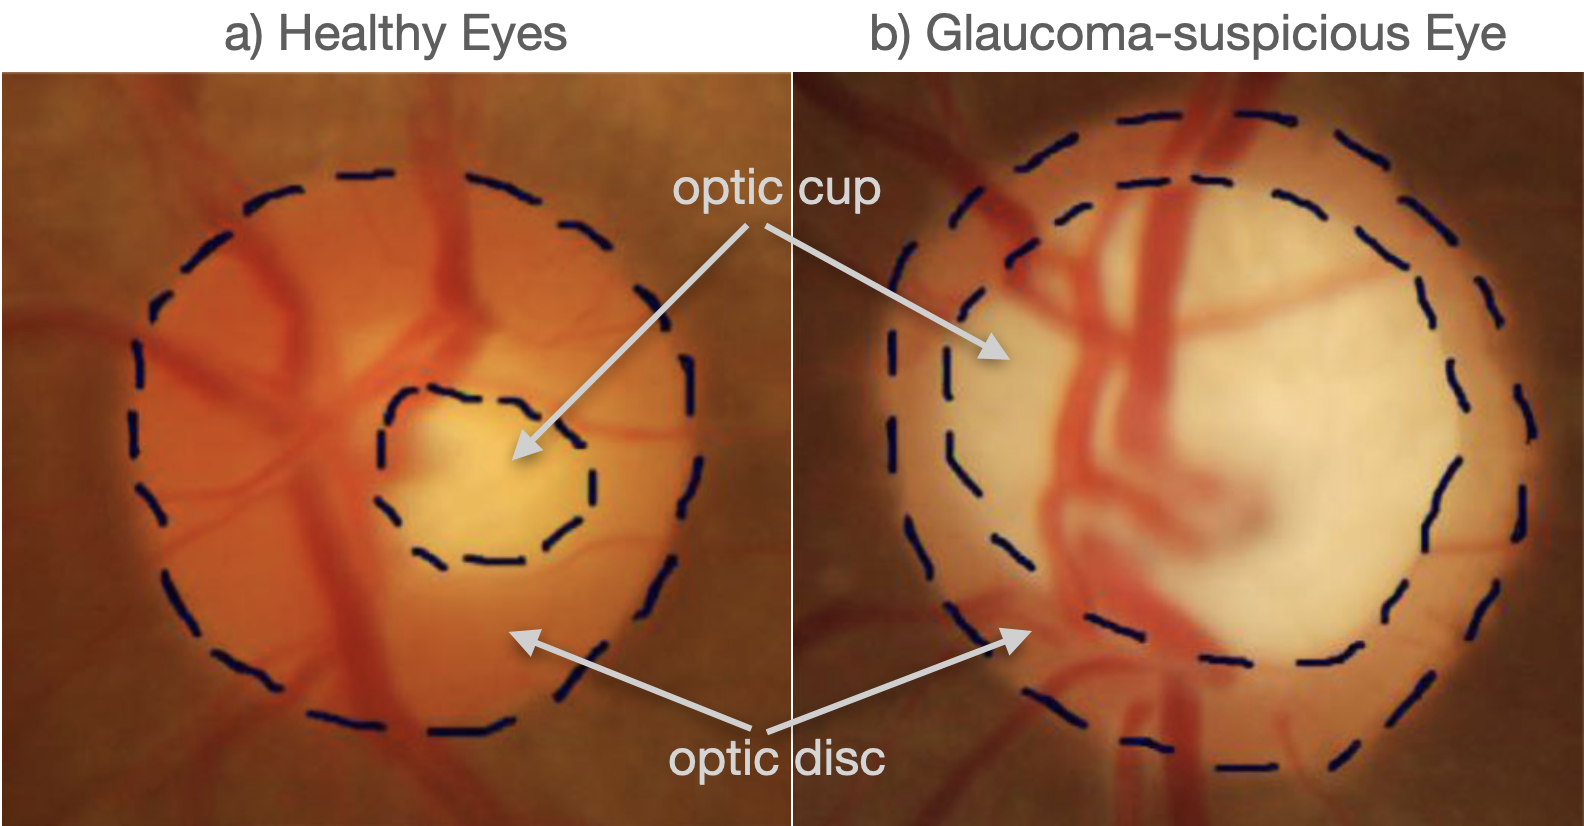
\includegraphics[width=0.5\textwidth]{assets/healthy-glcucoma}}
\caption{Fundus images representing a healthy and a glaucoma suspicious eye. The lines encapsulate the boundary of the optic disc and cup. The CDR of a glaucoma suspicious eye is larger than a healthy eye.}
\label{fig_eye}
\end{figure}

A popular segmentation deep learning network is U-Net\cite{ronneberger2015u}, an efficient, fully convolutional neural network for biomedical image segmentation. The success of U-Net has inspired many adaptations such as the Attention U-Net\cite{oktay2018attention}, and UNet++\cite{zhou2018unet++}. Their results have shown consistent improvement in segmentation performance over U-Net across various datasets in their studies. In this study, we will review and compare the performance of U-Net, Attention U-Net, and UNet++ to segment the optical disc and cup jointly.

\section{U-Net Architectures}

\subsection{U-Net}

In 2015, Ronneberger et al. introduced the U-Net\cite{ronneberger2015u} architecture. It consists of a contraction path (encoder) and an expansion path (decoder), as shown in Fig.~\ref{fig_unet}.

\begin{figure}[h]
\centerline{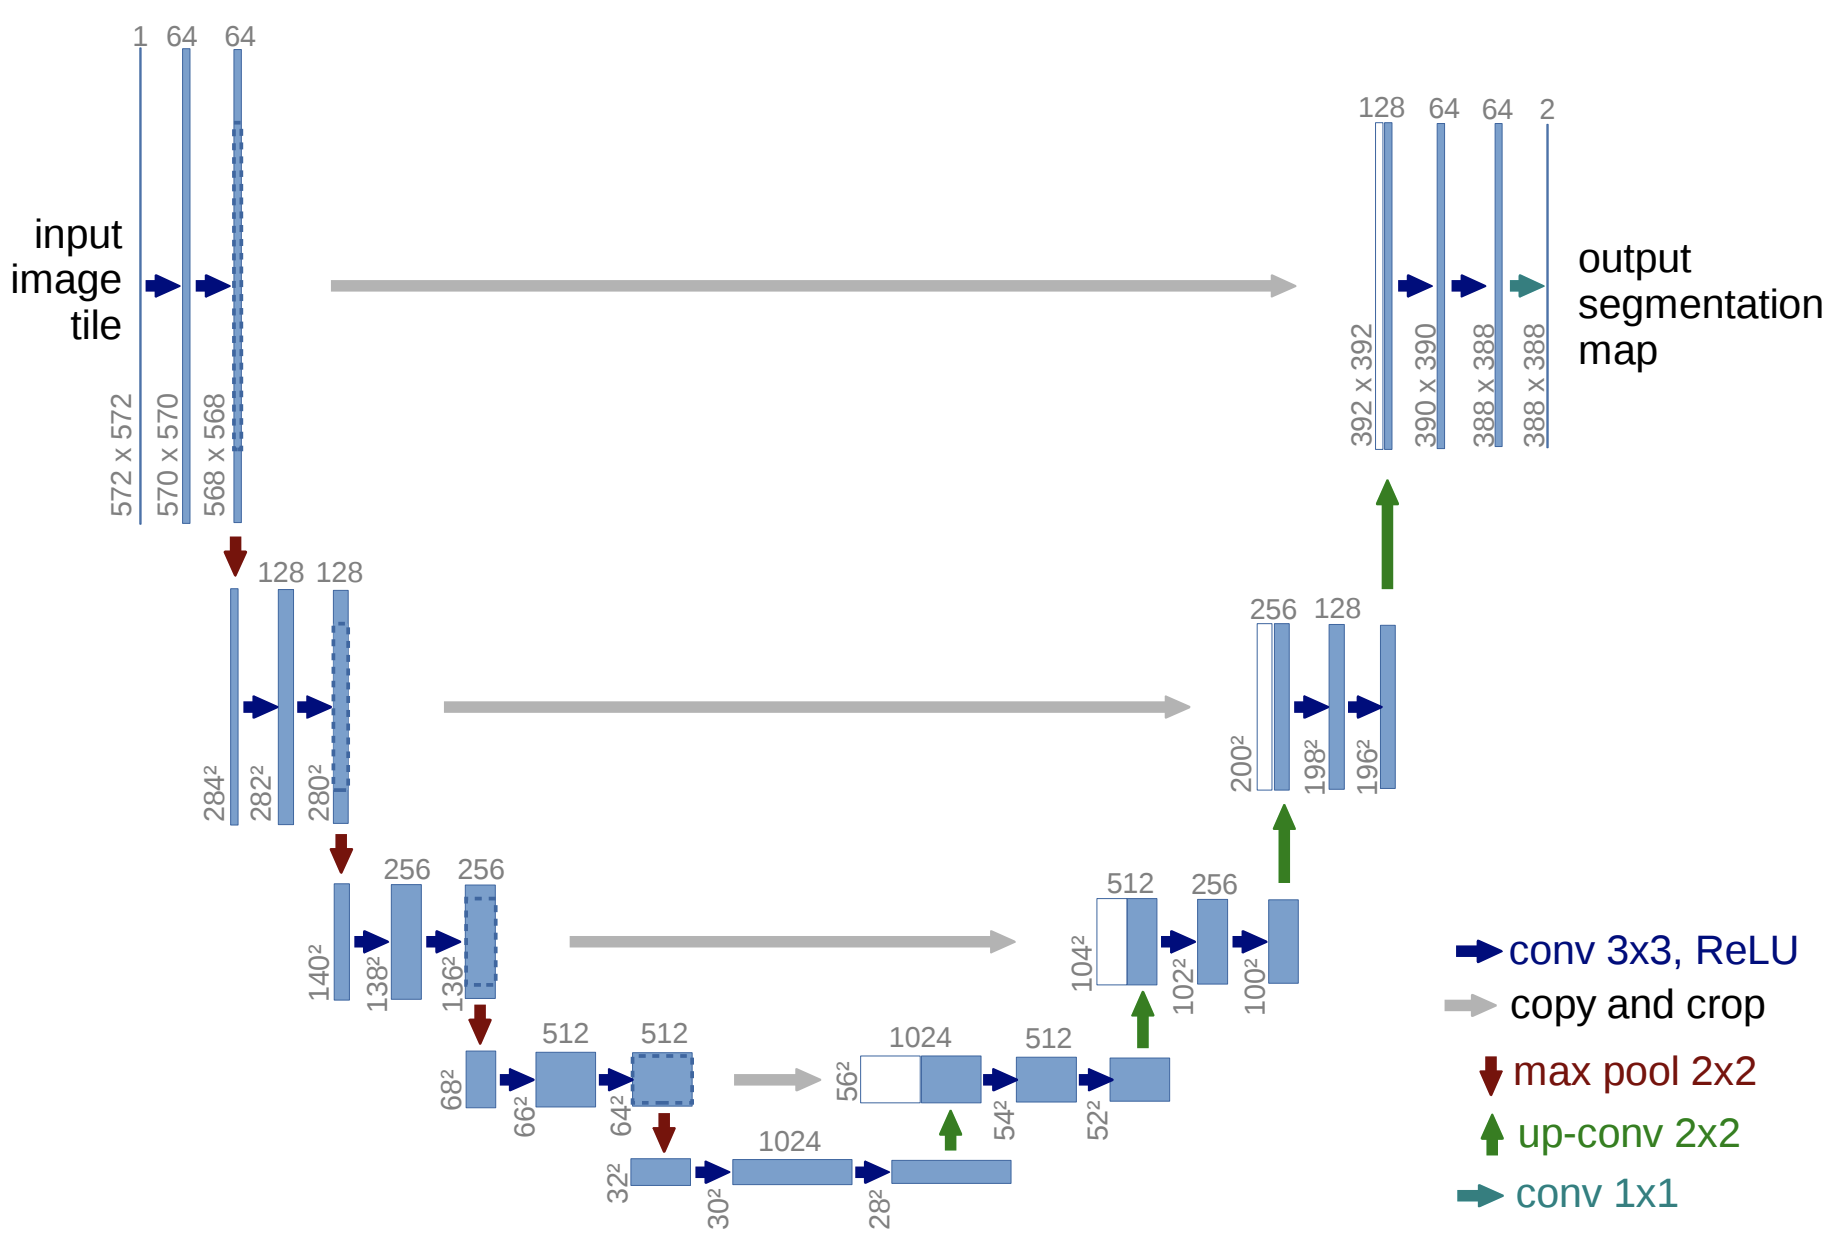
\includegraphics[width=0.5\textwidth]{assets/model-unet}}
\caption{U-Net, contracting path to capture context and a symmetric expanding path that enables precise localization.}
\label{fig_unet}
\end{figure}

The contraction path has a typical CNN architecture where it consecutively stacks two 3x3 convolutions followed by a 2x2 max pooling. This process downsamples the input at each step and doubles the number of feature maps. Element-wise rectified-linear non-linearity (ReLU) activation function is utilized.

The expansion path also utilizes a series of convolutional layers to output segmentation masks. 2x2 up-convolution performs upsampling from previous layers. The skip connections transfer the corresponding feature map from the contraction path and concatenate them to up-sampled decoder feature maps. This provides localization information from contraction path to expansion path, due to the loss of border pixels in every convolution. After two 3x3 convolutions, follow the 2x2 up-convolution layer. At each upsampling step, the number of feature maps is halved.

Finally, a classifier utilizes a 1×1 convolutional layer with sigmoid activation as the pixel-wise classification to produce the disc probability map.

In their study, they applied the U-Net to different segmentation tasks, including neuronal structures in electron microscopic recordings and cell segmentation tasks in light microscopic images. Their work won the ISBI cell tracking challenge 2015 by a large margin, achieving an average Intersection over Union of 77.5\%, which is significantly better than the second-best algorithm with 46\%. U-Net was released on the 2015 MICCAI and has gradually become the baseline for most medical semantic segmentation tasks.

\subsection{Attention U-Net}

Oktay et al. borrowed the idea of an end-to-end-trainable attention module\cite{jetley2018learn}, which is commonly used in natural image analysis. These attention maps can amplify the relevant regions, demonstrating superior generalization over several benchmark datasets, resulting in a more accurate and robust image classification performance.

\begin{figure}[h]
\centerline{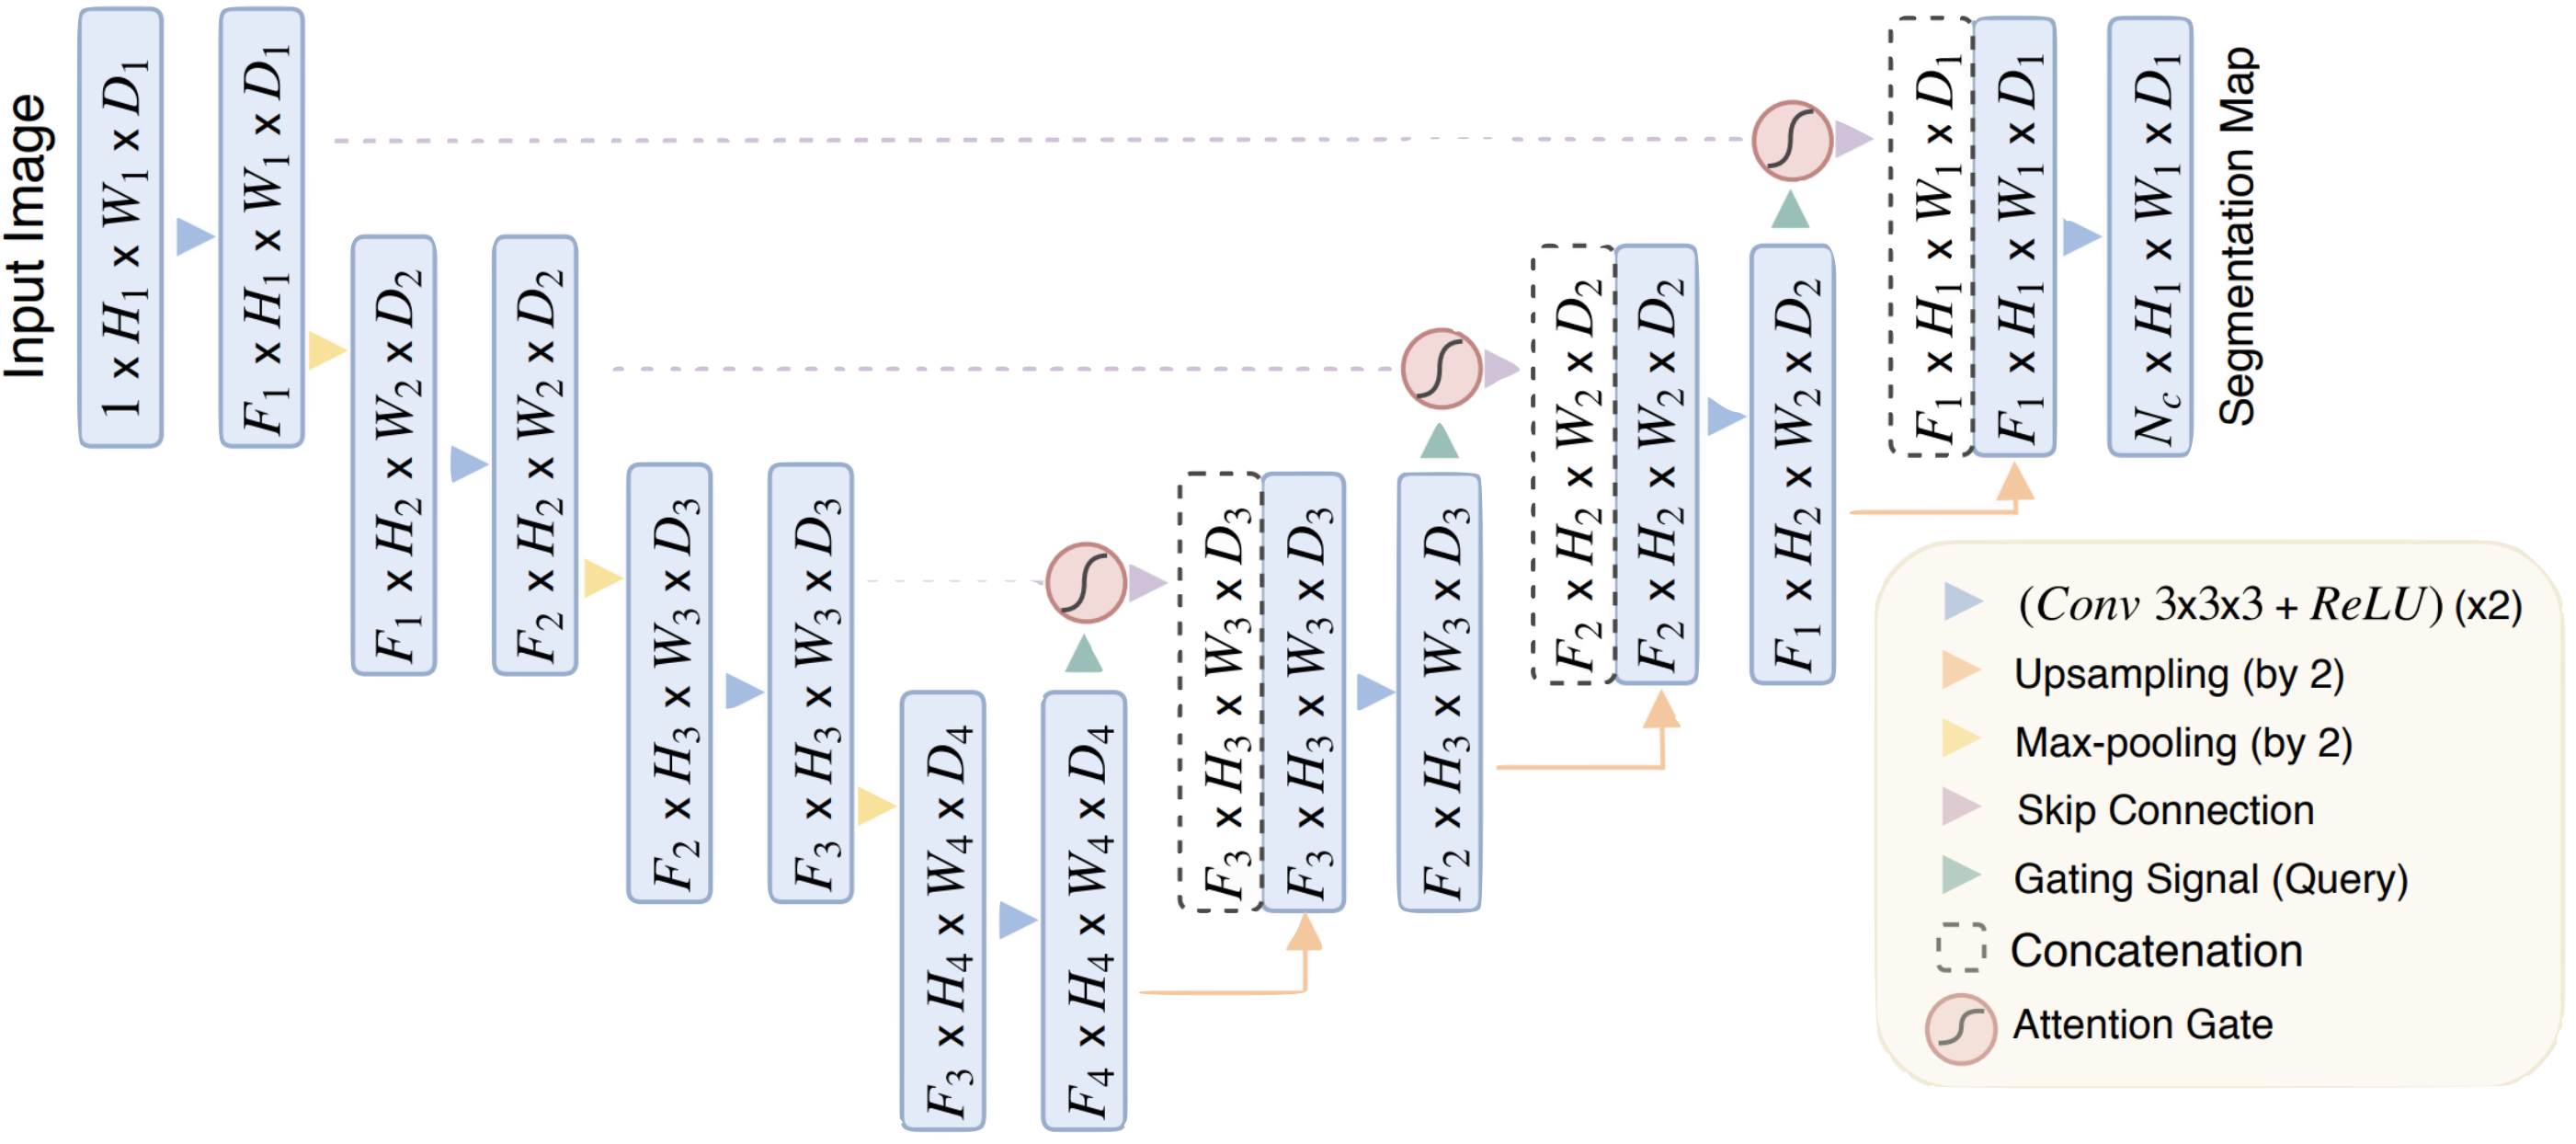
\includegraphics[width=0.5\textwidth]{assets/model-attention-unet}}
\caption{Attention U-Net, applying attention gates to suppress irrelevant regions in an input image while highlighting salient features.}
\label{fig_unet_attn}
\end{figure}

To improve segmentation performance, Khened et al.\cite{khened2019fully} and Roth et al.\cite{roth2018spatial} relied on additional preceding object localization models to separate localization and subsequent segmentation steps. This can be achieved by integrating attention gates on top of U-Net architecture without training additional models. As a result, attention gates incorporated into U-Net can improve model sensitivity and accuracy to foreground pixels without requiring significant computation overhead. Attention gates can progressively suppress feature responses in irrelevant background regions. Thus their approach eliminates the necessity of applying an external object localization model.

The attention gates are implemented before concatenation operation to merge only relevant activations. Gradients originating from background regions are down-weighted during the backward pass. This allows the model's parameters in prior layers to be updated based on spatial regions that are relevant to a given task.

To further improve the attention mechanism, Oktay et al. proposed a grid-attention mechanism. The gating signal is not a single global vector for all image pixels by implementing grid-based gating, but a grid signal conditioned to image spatial information. The gating signal for each skip connection aggregates image features from multiple imaging scales. Using grid-based gating allows attention coefficients to be more specific to local regions as it increases the grid-resolution of the query signal. This achieved better performance compared to gating based on a global feature vector.

In their study, they applied Attention U-Net on two different CT abdominal datasets, where segmentation is difficult due to pancreas shape-variability and poor tissue contrast. They benchmarked Attention U-Net against both the standard U-Net architecture, as well as the U-Net with an additional 8\% capacity. Their results demonstrated that Attention U-Net consistently outperformed U-Net in various datasets and model configurations.

\subsection{UNet++}

Zhou et al. aimed to improve segmentation accuracy with UNet++ by incorporating a series of nested, dense skip pathways between the encoder and decoder, and included a deep supervision method.

\begin{figure}[h]
\centerline{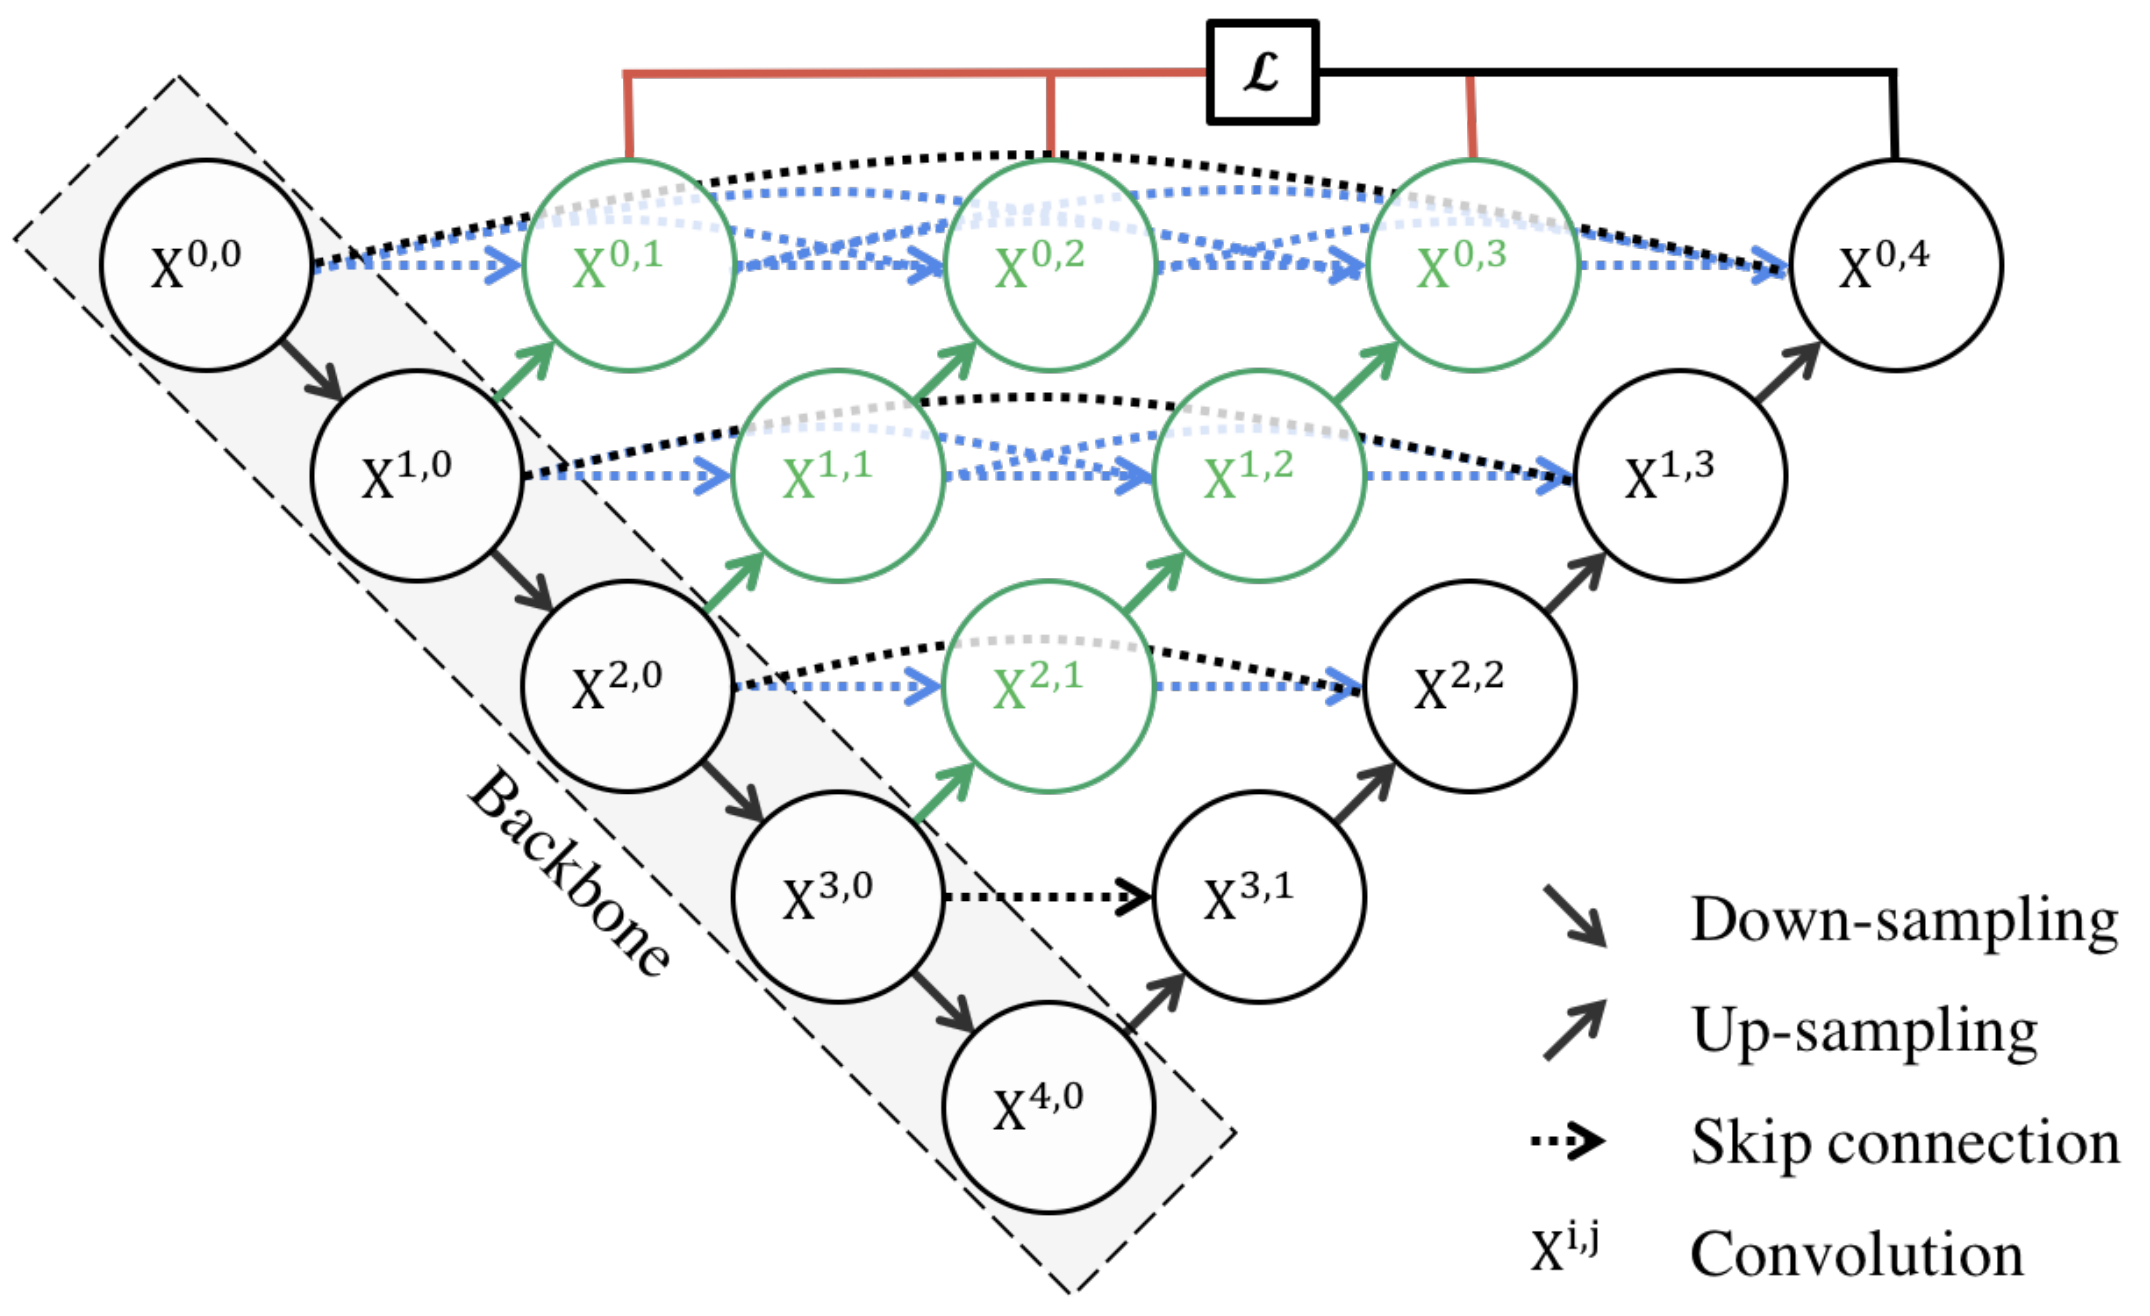
\includegraphics[width=0.5\textwidth]{assets/model-nested-unet}}
\caption{UNet++, re-designed skip pathways aim at reducing the semantic gap between the feature maps of the encoder and decoder.}
\label{fig_unet_nested}
\end{figure}

The redesigned skip pathways have been added to bridge the semantic gap between the encoder and decoder subpaths. The purpose of these convolution layers is to reduce the semantic gap between the feature maps of the encoder and decoder subnetworks, allowing the network to converge. U-Net's skip connections directly connect the feature maps between encoder and decoder, which results in fusing semantically dissimilar feature maps. However, with UNet++, the output from the previous convolution layer of the same dense block is fused with the corresponding up-sampled output of the lower dense block. This brings the semantic level of the encoded feature closer to that of the feature maps waiting in the decoder; thus, optimization is easier when semantically similar feature maps are received.

Dense skip connections have implemented skip pathways between the encoder and decoder. These Dense blocks are inspired by DenseNet\cite{huang2017densely} with the purpose to improve segmentation accuracy and improve gradient flow. Dense skip connections ensure that all prior feature maps are accumulated and arrive at the current node because of the dense convolution block along each skip pathway. This generates full resolution feature maps at multiple semantic levels.

Deep supervision is added so that the model can be pruned to adjust the model complexity, to balance between speed and performance. For accuracy, the output from all segmentation branches is averaged. For speed, the final segmentation map is selected from one of the segmentation branches.

In their study, they evaluated UNet++ across four medical image segmentation tasks. They reported that their methods had outperformed U-Net on average by 3.9\% in Intersection over Union. Deep supervision also enables more accurate segmentation, as UNet++ with deep supervision exhibits an average improvement of 0.6\% over UNet++ without deep supervision.

\section{Methods}

\subsection{Data}

As the datasets used in the U-Net, Attention U-Net, and UNet++ studies are various medical imaging datasets for model evaluation, we picked another medical imaging dataset, DRISHTI-GS1\cite{sivaswamy2014drishti}. 

DRISHTI-GS1 dataset is an open-access dataset by the International Institute of Information Technology, collected and annotated by Aravind Eye Hospital in India. This dataset is meant for validating the results of the optic disc and cup segmentation. It is divided into training and testing sets consisting of 50 and 51 fundus images, respectively. Selected patients were between 40 to 80 years of age, with a roughly equal number of males and females. 

The dataset contains two masks, one for the optic disc and another optic cup. Each input image has three channels, and the image size has been downsampled to 224 by 224. In our experiment, our goal is to compare optic disc and cup segmentation performance of various models. 

\subsection{Metric}

This study uses a set of metrics to compare model segmentation performance; 1) Binary Cross-Entropy, 2) Dice Coefficient, and 3) Intersection over Union.

\textbf{Binary Cross-Entropy (BCE)}. A common metric and loss function for binary classification for measuring the probability of misclassification. In a multi-label classification task, an element belonging to a certain class should not influence another class's decision. We need to compute the cross-entropy on top of each point's probabilities associated with the true class.

\textbf{Dice Coefficient (Dice)}. A metric measure of overlap between the predicted and the ground truth is often used to quantify image segmentation methods' performance. Dice measure how similar the objects are, where the size of the two segmentations' overlap is divided by the total size of the two objects. This metric ranges between 0 and 1, where a 1 denotes perfect and complete overlap.

\begin{equation}
\mbox{Dice Coefficient} = \frac{2 |A \cap B|}{|A| + |B|}
\end{equation}

\textbf{Intersection over Union (IoU)}. A simple yet effective metric to calculate how accurate the predicted mask is with the ground truth mask. It is a method to quantify the percent overlap between the target mask and our prediction output. It measures the number of pixels common between the target and prediction masks divided by the total number of pixels present across both masks. Similar to the Dice coefficient, this metric ranges from 0 to 1, where 0 signifies no overlap, whereas 1 signifies perfectly overlapping between predicted and ground truth.

\begin{equation}
\mbox{Intersection over Union} = {{|A \cap B|}\over{|A \cup B|}}
\end{equation}

\subsection{Training Protocol}

Each model was trained for 100 iterations with a minibatch size of 16, limited by the GPU memory. We used Adam optimizer with an initial learning rate value of 0.001 and reduced the learning rate when the loss metric has stopped improving after ten epochs by a factor of 10. L2 penalty was added to reduce overfitting by fixing 0.05 to weight decay. The loss function is a combination of the Binary Cross-Entropy loss and the Dice Coefficient loss. The models were trained on NVIDIA GeForce RTX 2080 Ti, and the training time per epoch was recorded.

Since the dataset is already split into training and test sets, we will train the model and validate the performance with each dataset, respectively. But due to the stochastic nature of machine learning, the performance of each method can be affected by the randomness in data shuffle, randomness in weights initialization, and randomness in GPU. To facilitate better comparison, we will train and validate each method with 30 randomly selected seed numbers. The reported performance of each method is the average result of all 30 runs.

Implementation and experiments for this study are built on the PyTorch framework and are made publicly available at a companion website\footnote{\href{https://github.com/jinglescode/meditorch/blob/master/demo/Drishti-compare-unet-atten_unet-nested_unet-30runs.ipynb}{github.com/jinglescode/meditorch}.}.

\section{Results and Discussion}

\begin{figure*}[ht]
\centerline{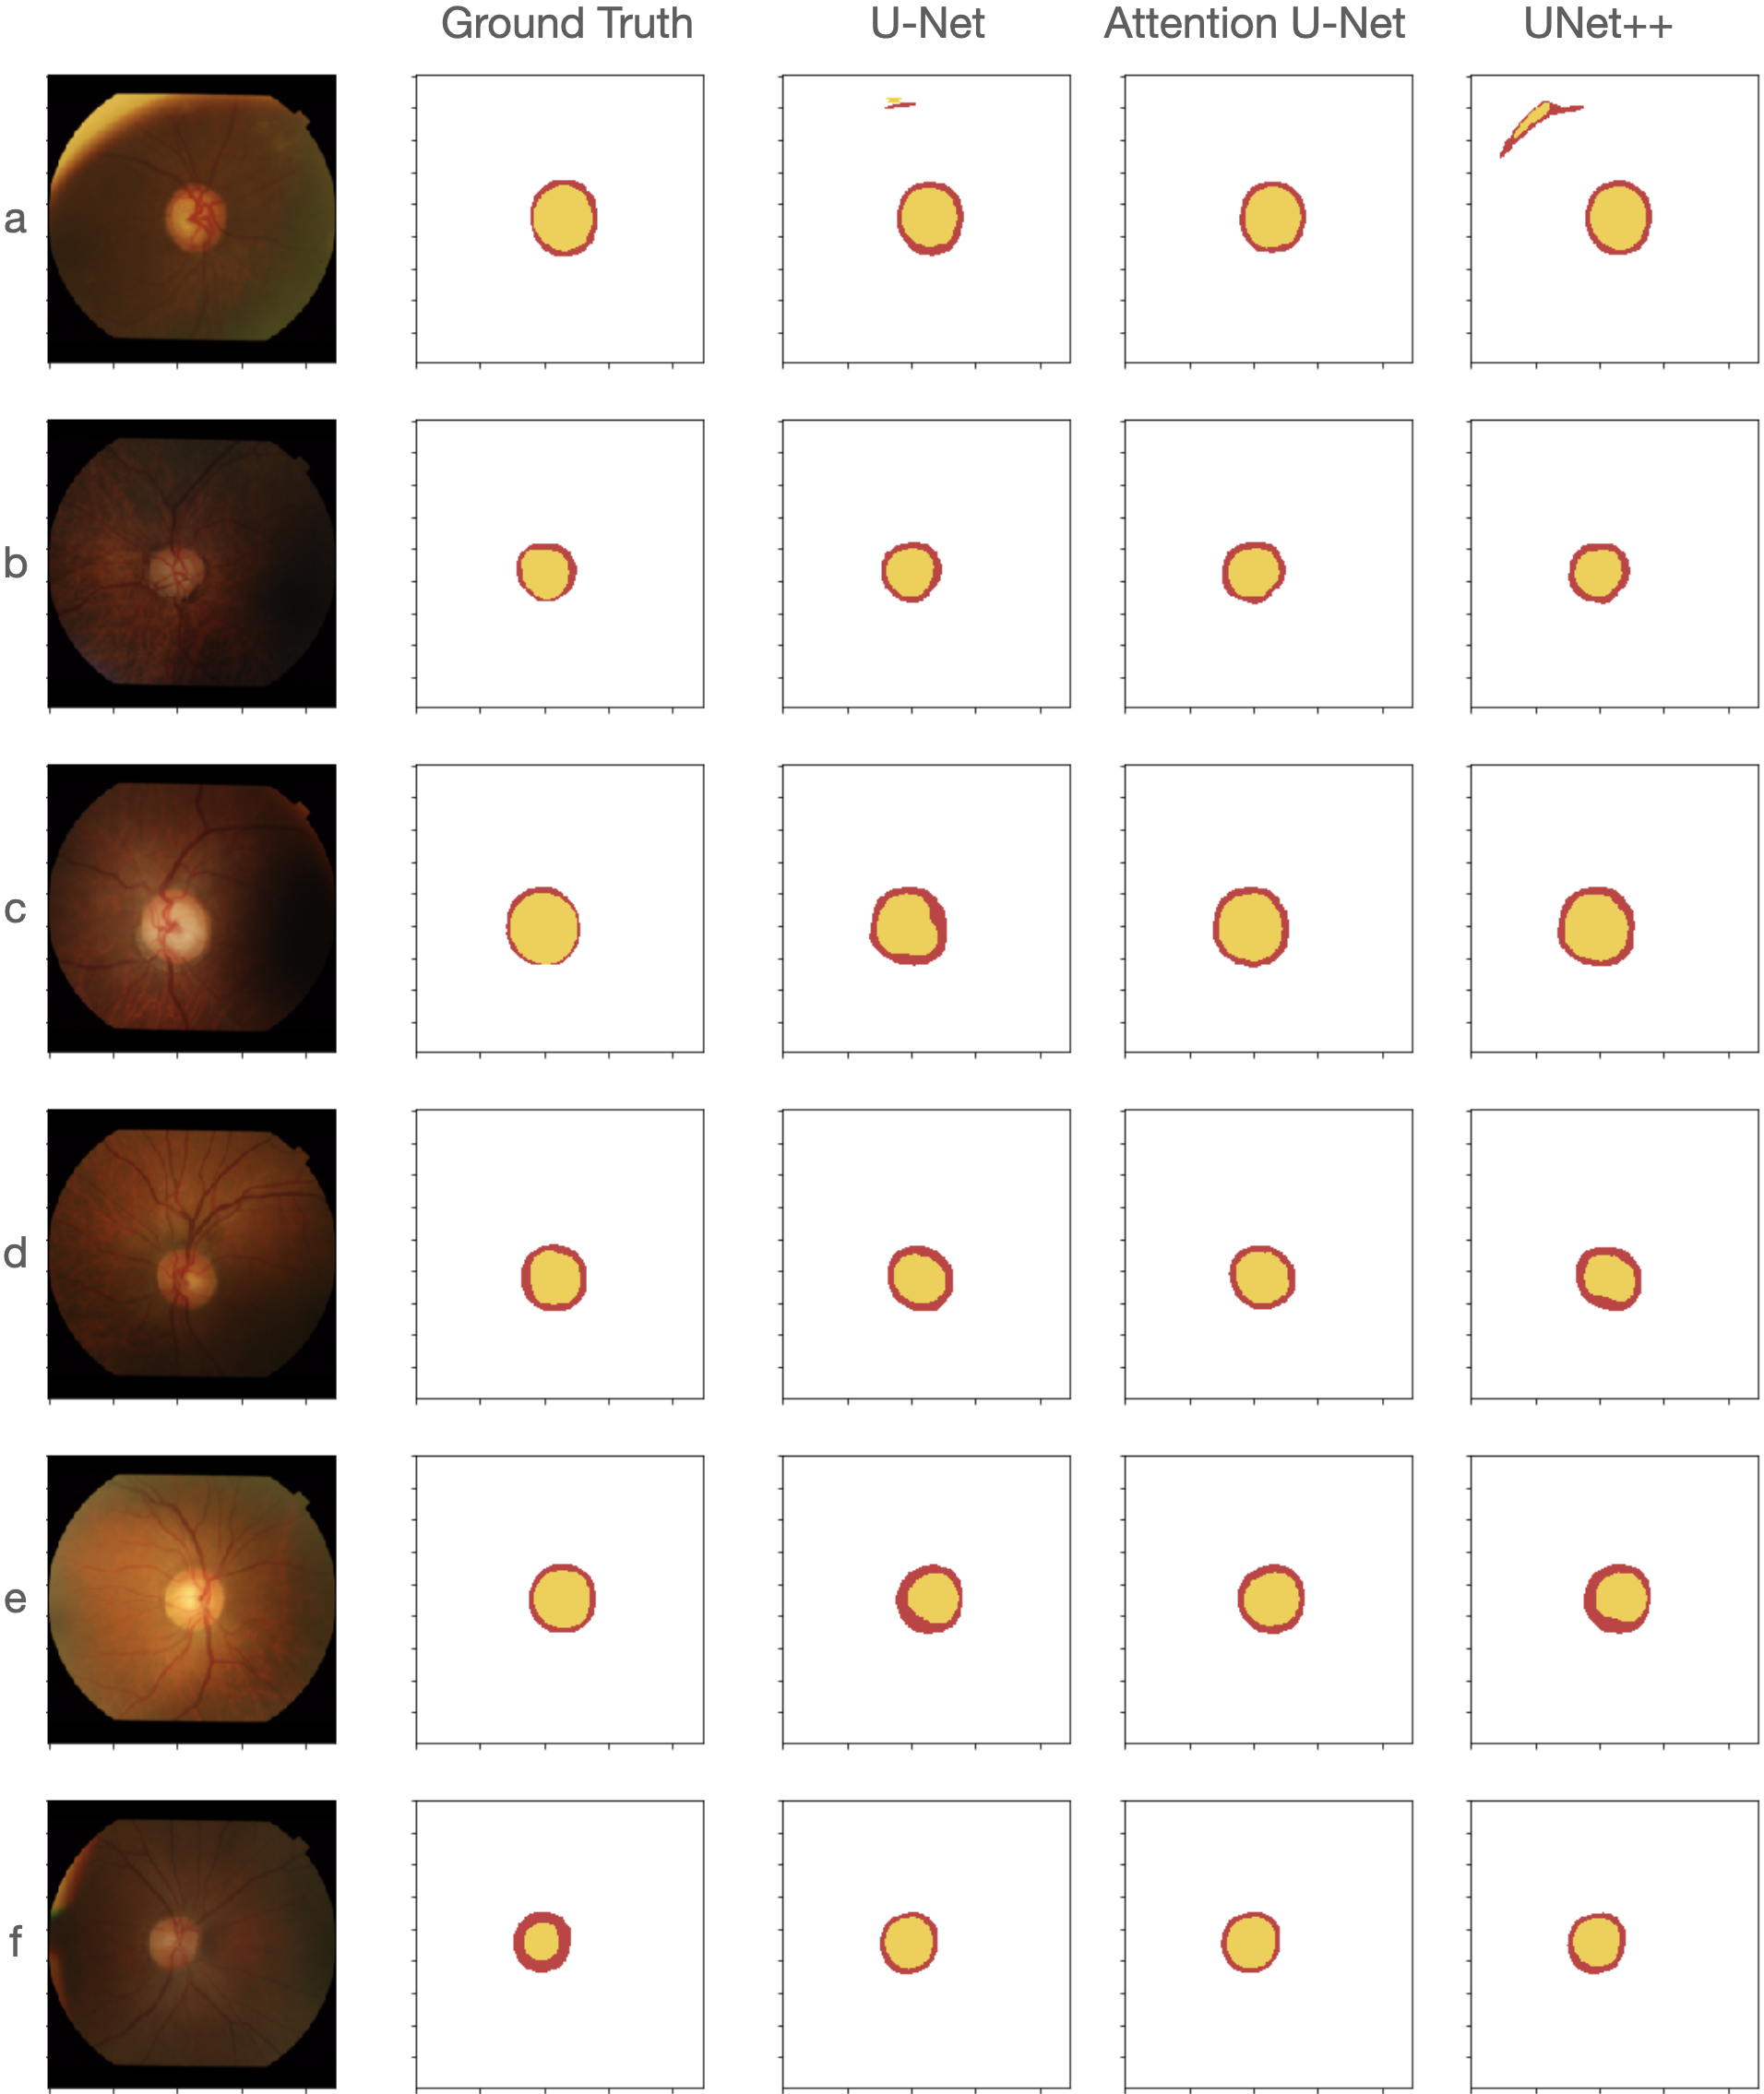
\includegraphics[width=1\textwidth]{assets/segmentations}}
\caption{Segmentation results, where the optical disc and optical cup are denoted as red and yellow, respectively.}
\label{fig_segmentations}
\end{figure*}

\begin{table}[t]
\centering
\caption{Performance of various methods}
\begin{tabular}{||c|c|c|c||}
\hline
\textbf{Model} & \textbf{\# Params} & \textbf{IoU} & \textbf{Time per Epoch} \\
\hline
U-Net & 34.5M & 0.873 & 2s \\
Attention U-Net & 34.8M & 0.868 & 3s \\
UNet++ & 36.6M & \textbf{0.878} & 5s \\
\hline
\end{tabular}
\label{table_results}
\end{table}

The segmentation performance of various U-Net architectures are shown in Table~\ref{table_results}. All the above-reported results are based on ground truth segmentation, and we average the IoU of 30 runs for all three architectures. Overall, all three architectures' segmentation performance is marginally close, with UNet++ best performing at 87.8\%. 

As Ronneberger has designed U-Net specifically to perform image segmentation on biomedical images, U-Net achieves good performance and good training time. U-Net is the smallest model, approximately 6\% smaller than UNet++. U-Net also performs training and inference faster, approximately half the time of UNet++.

In many deep learning research work, many researchers increases the model size to meet the needs of higher precision. Given that UNet++ has approximately 2 million more parameters and trains twice the time needed for original U-Net, this is demanding in computational resources and memory. It makes one wonder whether adopting this method is worth it, comparing the gains with its costs. 

To compare cup and disc segmentation performance visually, the predicted segmentation masks are shown in Fig.~\ref{fig_segmentations}, where the optical disc and optical cup are denoted as red and yellow, respectively. The samples were chosen to provide examples of over and underexposed images, commonly found in the real world. \textit{Image A} contains a shade of yellow on the top left corner; this is tricky for UNet++ as it has identified it as an optical disc and cup. \textit{Image B and F} are poorly lit, where it is difficult to separate the disc from the cup, but all three models were able to perform segmentation effectively. 

Nevertheless, these methods are able to identify discs and cups in most cases, and were able to generalize to different lighting conditions and subjects. This ability to generalize is critical for real-world application as we need models trained to perform disc and cup segmentation on other subjects, without fine-tuning or calibration.

\section{Conclusion}

Clinicians rely on the cup to disc ratio to quantify glaucomatous deformations, but identifying optical cups and discs is performed by trained glaucoma specialists. An algorithm that provides high precision extraction of optical cups and discs is highly desired, as is the ability to accurately quantify glaucomatous deformations is dependent on the completeness and accuracy of the segmentation.

This study reviews and compares the performance of U-Net, Attention U-Net, and UNet++; on segmenting the optical disc and cup jointly for diagnosing glaucoma. These networks were designed to perform image segmentation on various medical images datasets. We used intersection over union to access the predicted mask's accuracy with the ground truth; the average intersection over union for all three architectures is marginally close. We show that these networks were robust and performed under various lighting conditions, commonly found in real-world datasets. These methods could potentially be useful for glaucoma diagnostics. 
  
\bibliographystyle{unsrt}
\bibliography{references}

\end{document}
